\documentclass[conference]{IEEEtran}
\IEEEoverridecommandlockouts
% The preceding line is only needed to identify funding in the first footnote. If that is unneeded, please comment it out.
\usepackage{cite}
\usepackage{amsmath,amssymb,amsfonts}
\usepackage{algorithmic}
\usepackage{graphicx}
\usepackage{textcomp}
\usepackage{xcolor}
\usepackage[english, brazil]{babel}
\def\BibTeX{{\rm B\kern-.05em{\sc i\kern-.025em b}\kern-.08em
    T\kern-.1667em\lower.7ex\hbox{E}\kern-.125emX}}
\graphicspath{{images/}}
\begin{document}

\title{Manutenção de Fatores Biológicos de Crescimento da Orquídea {\itshape{Phalaenopsis}} com Internet das Coisas}


\author{\IEEEauthorblockN{Leonardo Miranda Amaral}
\IEEEauthorblockA{\textit{Dept. Engenharia de Computação} \\
\textit{Centro Universitário IESB}\\
Brasília, Distrito Federal, Brasil}
\and
\IEEEauthorblockN{Felipe Rodrigues Araújo}
\IEEEauthorblockA{\textit{Dept. Engenharia de Computação} \\
\textit{Centro Universitário IESB}\\
Brasília, Distrito Federal, Brasil}
\and
\IEEEauthorblockN{Rafael Roriz Barbosa}
\IEEEauthorblockA{\textit{Dept. Ciência da Computação} \\
\textit{Centro Universitário IESB}\\
Brasília, Distrito Federal, Brasil}
\and
\IEEEauthorblockN{Daniel Anes Da Silva Almeida}
\IEEEauthorblockA{\centerline{\textit{ Dept. Ciência da Computação}} \\
\textit{Centro Universitário IESB}\\
Brasília, Distrito Federal, Brasil}
}

\maketitle

\selectlanguage{brazil}
\begin{abstract}
Tendo em vista a necessidade da presença e auxílio de pessoas, sejam jardineiros ou responsáveis pelas plantas e jardins, nota-se a necessidade da construção de sistemas que possam automatizar e contribuir para a manutenção dos fatores pré-colheita. O presente trabalho propõe-se a criar um sistema com Internet das Coisas, API e Aplicação móvel para manutenção dos fatores pré-colheita do objeto de estudo. 
\end{abstract}

\selectlanguage{english}
\begin{abstract}
In view of the need of presence and help from people, whether gardners or the responsibles for the plants and gardens, the need for construction of automated systems is noticed to contribute for the maintaince of pre-harvest factors. A system using Internet of Things, an API and a Mobile Application for the maintaince of pre-harvest factors of the study object is proposed in the present work. 
\end{abstract}
\begin{IEEEkeywords}
Biology, Intelligent Garden, Microcontroller, Internet of Things, Sensors.
\end{IEEEkeywords}


\section{Introdução}

Automação é a denominação dada para sistemas automáticos de controle, pelos quais os mecanismos verificam seu próprio funcionamento, efetuando medições e introduzindo correções sem a necessidade da interferência humana. Atualmente, a automação está presente em diferentes níveis de atividades do homem, desde as residências até processos industriais.

A internet das coisas, ou como mais conhecida do inglês, Internet of Things (IoT), é a técnica de se utilizar tecnologias embarcadas em objetos do dia a dia, como utensílios domésticos e equipamentos eletrônicos em geral, conectando-os à internet e trocando informações com outros objetos, usuários e servidores, com vistas a determinado objetivo.

Tal plataforma permite impactar positivamente no uso dos recursos de monitoramento e automação aplicados no jardim, que geralmente consiste em um microcontrolador central ao qual outros objetos estão conectados. O jardim inteligente consiste em um microcontrolador como hub para diferentes tipos de sensores, como sensor de umidade, sensor temperatura, tanto do solo como do ar, e bomba d’água para irrigação.

Quando as pessoas tentam fazer plantações e montar seu próprio jardim, tais plantas como a Orquídea {\itshape{Phalaenopsis}} que é objeto de pesquisa podem demandar cuidados especiais e constantes nos seus estágios iniciais ou durante toda a vida da planta. Porém, com o passar dos dias, devido à falta de manutenção, pode ocorrer da planta não sobreviver.

O microcontrolador enviará os dados via o serviço MQTT Cloud Service para uma API REST. Um aplicativo de computação móvel fará requisição dos dados da API REST utilizando protocolo HTTP. Tal aplicativo de computação móvel vai fornecer ao usuário as informações de temperatura e umidade, e o gerenciamento do sistema de controle e manutenção da planta.

Este protótipo ajudará pessoas no monitoramento dos parâmetros e na manutenção do jardim, desempenhando um papel vital e servindo como um bom companheiro para as plantas.

Este artigo está organizado da seguinte forma: Seção 1 a 3: Apresentação de uma abordagem de tratamento de plantas com base nas tecnologias apresentadas. Seção 4 a 5: Objetivos e formas de aplicação do projeto. Seção 6: Metodologia e estudos da planta objeto de pesquisa Orquídea Phalaenopsis, e documentação dos métodos utilizados, assim como também apresentação dos componentes a serem utilizados na construção do sistema. Seção 7: Implementação dos componentes e tecnologias na construção do sistema. Seção 8: Trabalhos correlatos. Seção 9: Metodologia utilizada. Seção 10: Resultados obtidos. Seção 11: Conclusões.

\section{Contextualização}

 Na atual era de tecnologia, a automação é a chave para o crescimento de vários setores da economia. Desde manufatura e agricultura até serviços e logística podem ser melhorados por meio da tecnologia. Ao utilizar a internet das coisas que é a técnica de usar poder computacional para monitorar e controlar alguns parâmetros do dia a dia. Novos sistemas estão sendo desenvolvidos fazendo uso de sensores, softwares e protocolos de comunicação para automatizar tarefas específicas. Atualmente, algumas pessoas preferem ter seus próprios jardins ou outras pequenas árvores de frutas em suas residências. Muitas vezes, precisam ser cautelosas durante os estágios iniciais de crescimento. Como resultado, o jardim pode eventualmente ser destruído por uma pequena falta de atenção. Também, condições climáticas podem favorecer o encurtamento da vida do jardim. Pois, algumas plantas podem morrer devido a falta de umidade, falta de incidência solar ou calor intenso.

\section{Problematização}
Devido a planta usada como objeto de estudo demandar elevado cuidado e atenção. Porém, ao faltar estes pode fazer com que a planta morra. Mas quais fatores biológicos  são importantes de serem compreendidos e em como afetam o desenvolvimento da Orquídea {\itshape{Phalaenopsis}}? Como  alguns destes fatores podem ser supridos com pouca necessidade da atenção humana? Como o sistema pode ser feito de forma resiliente?

\section{Objetivo geral}
Criar um sistema resiliente composto de sensores, um microcontrolador, um aplicativo móvel e uma API para auxiliar o usuário no controle de alguns dos fatores a serem compreendidos neste trabalho para o desenvolvimento da Orquídea {\itshape{Phalaenopsis}}.

\section{Objetivos específicos}
\begin{itemize}
    \item Conhecer os requisitos de umidade, intensidade de luz e temperatura da Orquídea {\itshape{Phalaenopsis}};
    \item Fazer uso de sensores para detectar umidade e temperatura tanto do ar como do solo, e intensidade de luz conectado a um microcontrolador;
    \item Fazer o sistema de controle de umidade conectado ao microcontrolador;
    \item Fazer o sistema de controle de temperatura conectado ao microcontrolador;
    \item Fazer o sistema de controle de luminosidade conectado ao microcontrolador;
    \item Criar uma API REST para coletar dados e armazenar no banco de dados;
    \item Enviar os dados do microcontrolador utilizando o serviço MQTT Cloud Service para a API REST;
    \item Baseado nos parâmetros definidos pelo usuário, a API utiliza o microcontrolador para acionar os sistemas de controle de temperatura e umidade;
    \item O aplicativo de computação móvel faz a requisição desses dados para a API REST utilizando o protocolo HTTP para que sejam fornecidos para o usuário, além de enviar configurações dos sistemas de controle de umidade e temperatura.
\end{itemize}

\section{Referencial teórico}
\subsection{Biologia}
Conhecer os aspectos biológicos da planta contribui para o seu melhor cuidado. A Floricultura, são todas as plantas ornamentais sem ramos lenhosos, incluindo plantas de canteiro e de jardim, anuais ou perenes, flores de corte, ramagens de corte, plantas floríferas em vaso, plantas de folhagem para uso em interiores e material de propagação, e é um ramo da agricultura em que se lida com o cultivo de flores. A indústria da floricultura a cada dia cresce mais. Esta abrange múltiplas formas de exploração e cultivo, assim como: flores de corte, flores secas, flores e plantas em vaso, folhagens, mudas, plantas ornamentais, bulbos, tubérculos, rizomas, estacas e sementes.
O objeto de estudo se encaixa em Flores de Corte, também conhecidas como Cut Flowers. As flores podem ser frescas, secas ou preservadas, vendidas em forma de haste, ramalhetes ou arranjos.\cite{b2,b1}

Contudo, as flores de corte são vulneráveis a altas perdas pós-colheita. O manuseio de pós-colheita é um processo que começa no nível da fazenda, onde se inicia sua plantação. Devido a isto, torna-se importante o conhecimento do manuseio das flores de forma apropriada para mantimento de sua qualidade e frescor. É difícil determinar a vida pós-colheita de uma flor, pois, é influenciada por diversos fatores {\itshape{viz.}}, Fatores pré-colheita, Estágio de colheita e Fatores pós-colheita.\cite{b1}

No entanto, como o foco deste trabalho é a qualidade do mantimento e vida da planta, apenas abordaremos os Fatores pré-colheita. Diversos são os fatores pré-colheita, e podem ser classificados como ambientais e culturais.
Nos fatores (ou práticas) ambientais pré-colheita se encaixam: temperatura, umidade relativa do ar, luminosidade, textura do solo, vento, altitude e chuva. Nos fatores (ou práticas) culturais se incluem: nutrição mineral, manejo do solo, poda, raleio, aplicações de produtos químicos, uso de porta-enxertos, espaçamento do plantio, irrigação e drenagem.\cite{b3}

O escopo deste trabalho irá abordar os seguintes fatores como objetos de estudo: intensidade de luz, temperatura, e umidade do solo e ar.

\subsubsection{Intensidade de Luz}
A intensidade de luz, também conhecida como luminosidade é um dos fatores mais importantes, pois está relacionada à fotossíntese, e é usada como fonte de energia pelas plantas. A luz ajuda na regulação de diversos processos fisiológicos. A luz também determina a quantidade de carboidratos nas plantas durante o crescimento em que influencia na qualidade de conservação. Plantas que contêm folhas suaves e flexíveis são plantas em que provavelmente são sensíveis a luz, e não deveriam ser colocadas em uma janela com muita radiação solar. A maioria das orquídeas preferem luz indireta ou luz filtrada com sombra. A Orquídea {\itshape{phalaenopsis}} necessita de luzes baixas (1200-2000 f.c.). \cite{b3, b1, b4, b5}

\subsubsection{Temperatura}
Geralmente, altas temperaturas resultam em altos níveis de respiração. A luminosidade e alta temperatura têm relação direta, e não podem ser tratados isoladamente, pois altas temperaturas têm uma forte associação com a exposição direta ao sol. A temperatura é fator determinante para muitos eventos fisiológicos, e está diretamente relacionada às suas propriedades qualitativas, como o conteúdo de açúcares nos frutos. O resfriamento é essencial para reduzir mudanças metabólicas como atividade enzimática e retardar a maturação da flor. A Orquídea {\itshape{Phalaenopsis}} é uma orquídea que pode ser classificada como orquídea de climas quentes ou tropicais, pois, ela necessita de temperaturas entre 24ºC e 30º graus durante o dia e temperaturas de 18ºC e 20ºC durante a noite. \cite{b3, b4, b5, b6, b7}

\subsubsection{Umidade}
A quantidade de vapor de água no ar representa a umidade. Isto ajuda na manutenção da temperatura da planta e no controle da perda de água da superfície da planta. Alta umidade resulta em alta fotossíntese. Em geral, as orquídeas requerem 80-85\% de umidade no ar para um crescimento satisfatório. A maioria das orquídeas preferem água com pH 5.0-6.5. A irrigação com baixo ou alto pH ou elevados níveis de minerais dissolvidos podem dificultar a retenção dos nutrientes. A água da chuva é o ideal. A Orquídea {\itshape{phalaenopsis}} pode ter uma melhor saúde com sua umidade do solo entre 50-70\% . \cite{b1, b4, b5, b6, b7}

\subsection{Hardware}
Além do software, o sistema proposto para se ter conhecimento dos fatores da Orquídea e auxiliar na sua vida possui componentes físicos e eletrônicos necessários para a contribuição ao projeto. A seguir serão discutidos os componentes físicos a serem utilizados.

\subsubsection{Microcontrolador}
Com o passar dos anos os microcontroladores começaram a ficar mais acessíveis e a serem usados para automatização de diversas áreas, como casas inteligentes, dispositivos vestíveis, monitoramento de qualidade do ar e diversas outras aplicações.
O ESP32 foi lançado no mercado em Setembro de 2016 pela Espressif Systems para substituir o ESP8266. O dispositivo ESP32 é um dispositivo poderoso com Wi-Fi e Bluetooth® já embutidos, feito para ser a solução perfeita para dispositivos IoT,\cite{b8} além de trazer elevado custo-benefício devido a já vir com as comunicações sem fio já embutidas. O ESP32 também possui um melhor processador em comparação a outros microcontroladores.\cite{b8}

O ESP32 mostrado na Fig.~\ref{fig:esp_32} irá ser utilizado com o Bluetooth® para poder se comunicar com o dispositivo móvel para a configuração inicial (Nome do dispositivo, Id do usuário, informações do Wi-Fi ao qual o dispositivo irá conectar, e credenciais do MQTT). Ademais, o ESP32 também é utilizado para a comunicação com o broker do MQTT, o HiveMQ, para passar os dados dos sensores e receber também. É necessário a utilização de sensores em conjunto com o microcontrolador para que possa ser feita a verificação dos parâmetros a serem abordados na planta.

\selectlanguage{brazil}
\begin{figure}
    \centering
    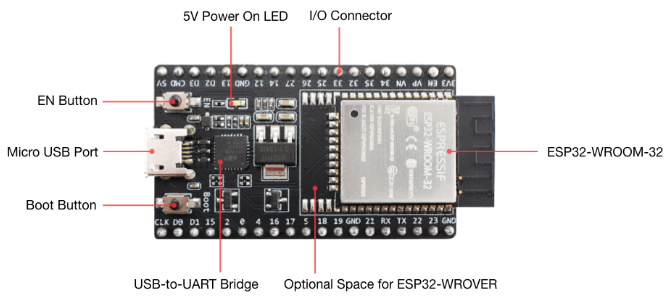
\includegraphics[width=8cm]{esp_32.png}
    \caption{Microcontrolador ESP32, conforme em \cite{b24}.}
    \label{fig:esp_32}
\end{figure}

\subsubsection{MQTT}
O protocolo MQTT é utilizado no presente trabalho para a comunicação do microcontrolador e a API para disponibilização dos dados e medições realizadas pelos sensores, assim como, o gerenciamento do módulo de controle. Este protocolo faz parte dos protocolos da camada de aplicação, sendo esta a responsável por prover serviços ao usuário final. Ele é baseado em um paradigma que permite a transmissão de mensagens para agrupamentos específicos de clientes de forma intermitente. Esse paradigma, conhecido como Publish-Subscriber, ou Publicador-Assinante, permite que clientes interessados passem a assinar tópicos de seu interesse em um servidor centralizado chamado Broker MQTT. Um broker pode conter múltiplos tópicos, onde cada um deles permite a recepção de mensagens de diferentes dispositivos publicadores e a entrega aos múltiplos dispositivos assinantes daquele tópico.\cite{b22}

\selectlanguage{brazil}
\begin{figure}
    \centering
    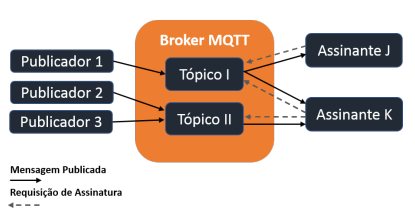
\includegraphics[width=8cm]{broker_mqtt.png}
    \caption{Comunicação por meio do paradigma Publicador-Assinante adotado pelo protocolo MQTT, conforme em \cite{b22}.}
    \label{fig:broker_mqtt}
\end{figure}

A Fig.~\ref{fig:broker_mqtt} mostra um cenário onde três dispositivos publicadores alimentam um broker que possui dois tópicos e dois assinantes. Neste cenário, o dispositivo Assinante J manifesta interesse nas mensagens provindas do Tópico I, o qual é responsável por propagar as mensagens advindas do dispositivo Publicador 1. O Assinante K, por sua vez, além de receber os dados publicados pelo dispositivo Publicador 1, por meio da assinatura ao Tópico I, recebe os dados publicados pelos Publicadores 2 e 3, por meio da assinatura ao Tópico II. Logo, sempre que um dispositivo publicador envia uma mensagem para o broker, tal mensagem é propagada para todos os dispositivos assinantes.\cite{b22}

Além dos conceitos citados de Assinante, Publicador e Tópico, é necessário compreender o conceito de níveis de Qualidade de Serviço, do inglês, Quality of Service levels (QoS). QoS é um acordo entre duas partes (remetente e destinatário) de uma mensagem no que diz respeito à garantia da distribuição dos dados. No protocolo MQTT são estabelecidos três diferentes níveis de QoS. No nível 0 de QoS, a mensagem é enviada uma única vez ou ainda não ocorrer, e não fornece garantia de entrega da mensagem. No nível 1 de QoS, existe a garantia de que a entrega ocorrerá, mas não há controle de entregas duplicadas, e a mensagem é enviada pelo menos 1 vez. No último nível, o nível 2 de QoS também possui garantia de entrega, porém, neste nível a duplicidade é eliminada e a mensagem é entregue exatamente uma única vez através de um handshake de quatro vias. \cite{b22,b23}

\subsubsection{Sensor de luminosidade}
O sensor a ser utilizado para incidência de luz será o TEMT6000 conforme apresentado na Fig.~\ref{fig:temt6000}. Este é um fototransistor NPN. O dispositivo é sensível ao espectro visível de luz e detecta a intensidade da luz. Adaptado a responsividade do olho humano. O sensor detecta o brilho do ambiente, e sua medida utilizada é a iluminância (lux). E funciona da seguinte forma: quanto maior a corrente, mais brilho está medindo e quanto menor a corrente, menos brilho está medindo, pois os fotodiodos convertem a luz em valores de corrente. Ângulo de sensitividade: 60°. \cite{b17, b18, b19} Porém, como o sensor utilizado mede em lux e a unidade de medida citada no artigo está em f.c., pode ser utilizada a conversão de 10.76 lux para 1 f.c.\cite{b20}

\selectlanguage{brazil}
\begin{figure}
    \centering
    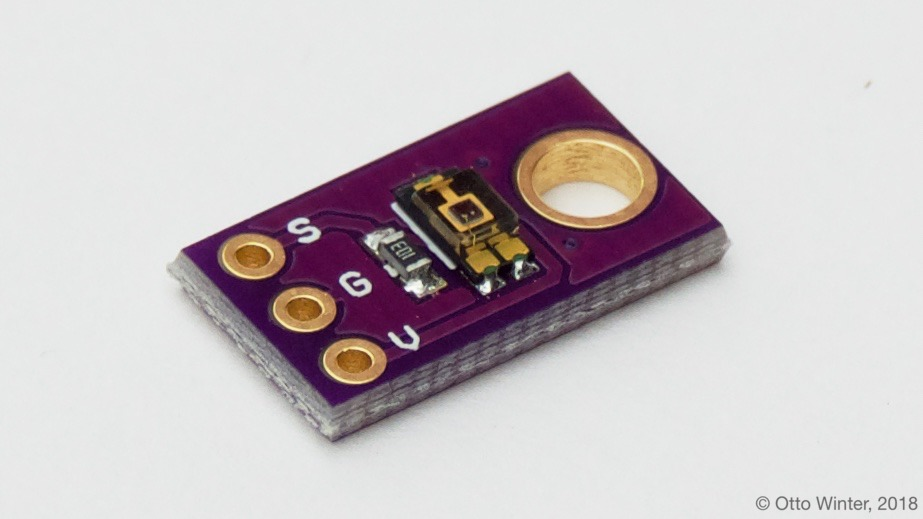
\includegraphics[width=8cm]{temt6000.jpg}
    \caption{Sensor TEMT6000, conforme em \cite{b25}.}
    \label{fig:temt6000}
\end{figure}

\subsubsection{Sensor de temperatura e umidade do ar}
O sensor de temperatura a ser utilizado será o DHT11 conforme apresentado na Fig.~\ref{fig:dht11}. Este é um sensor digital de baixo custo em que verifica-se a temperatura e a umidade do ar. O sensor é feito da seguinte forma: contém uma porção capacitiva sensitiva utilizada para a medição da umidade e um termistor para a detecção da temperatura. \cite{b9, b10}

\selectlanguage{brazil}
\begin{figure}
    \centering
    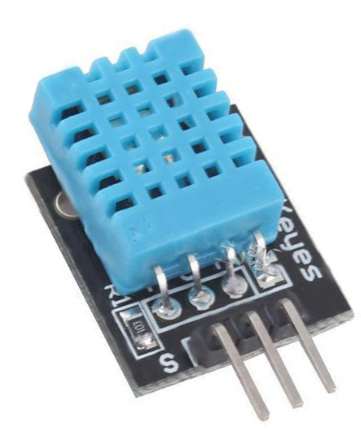
\includegraphics[width=5cm]{dht11.png}
    \caption{Sensor DHT11, apresentado em \cite{b26}.}
    \label{fig:dht11}
\end{figure}

\subsubsection{Sensor de umidade do solo}
O módulo de sensor de umidade do solo utilizado conforme apresentado na Fig.~\ref{fig:yl69} possui dois componentes, YL69 e YL38, em conjunto detectam o nível de umidade presente no solo. Essa medida ocorre com o nível de água presente no solo. É utilizada a propriedade de resistência elétrica do solo. A sensitividade é equivalente à diferença da água no solo; maior a quantidade de água no solo, maior é a condutividade e, como resultado, menor é sensitividade. \cite{b9, b10}

\selectlanguage{brazil}
\begin{figure}
    \centering
    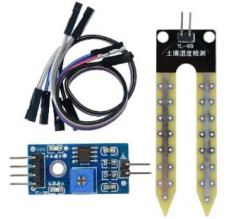
\includegraphics[width=5cm]{yl69.png}
    \caption{Sensor YL69 e YL38, apresentado em \cite{b27}.}
    \label{fig:yl69}
\end{figure}

\subsubsection{Módulo de controle}
Apesar de vários dos componentes utilizados no hardware e mais importantes serem os citados acima que correspondem ao monitoramento da planta, é importante de se ter conhecimento sobre os componentes a serem usados no módulo de controle. 

São componentes que podem ser encontrados com facilidade, sendo os seguintes: Uma bomba d'água para bombeamento da água para a planta, sendo utilizada para aumentar a umidade do solo da planta conforme os parâmetros utilizados pelo usuário; uma ventoinha responsável pelo aumento da umidade do ar, e uma lâmpada responsável pelo aumento da incidência de luminosidade da planta e de sua temperatura. Porém, esse sistema de controle é apenas uma abstração do que seria uma estufa para maior escala do sistema de controle.

\subsection{Software}
O Software faz-se necessário ao sistema devido a ser o meio usado para controle do microcontrolador e sensores, assim como armazenamento e relatação dos dados obtidos.

\subsubsection{API}
Os principais objetivos com o uso da API no sistema proposto são: fazer separação do backend e frontend, trazer possibilidade de consumo da aplicação, uso dos dados e comunicação com o microcontrolador por outras aplicações, descentralizar a aplicação de um único dispositivo e trazer maior disponibilidade de dados em tempo real. Além de ser o ponto principal da resiliência do sistema em questão, pois através dele ocorre a descentralização e modularização do sistema, e este está disponivel na nuvem através de uma PaaS (Platform as a Service) em uma instância privada, com isto tem se maior confiabilidade e menor gestão de infraestrutura, além de gerar maior rapidez no deploy da aplicação e numa possível queda da aplicação. E, tem-se também o banco de dados disponível em um cluster privado numa PaaS. Ao utilizar a nuvem para hospedagem de aplicação e banco de dados não quer dizer que não sofrerá falhas, mas conforme o design e arquitetura da infraestrutura a recuperação de falhas ocorrerá de forma mais rápida e será mais resistente a falhas.\cite{b28,b29}

A principal proposta das APIs (Application Programming Interface) é tornar disponível bibliotecas de código, SDKs, e frameworks para programadores.
O estilo arquitetural a ser usado para a API é o REST (Representational State Transfer). Nesta, busca-se seguir os seguintes padrões: sem estado (stateless), relacionamento client-server desacoplado, armazenável em cache, interface uniforme, sistema em camadas e opcionalmente prover código sobre demanda. \cite{b12, b13}

Outro padrão a ser utilizado por este projeto é o padrão de design MVC (Model-View-Controller) para a arquitetura da API. Este foi apresentado por Krasner e Pope no sistema Smalltalk \cite{b16}. Essas camadas, conforme as referências\cite{b14, b15}  propõem o seguinte: 
\begin{itemize}
    \item A Model é um objeto ou conjunto de objetos representando dados ou um processo como a base de dados, e processo de máquinas. Gerencia a informação na forma de dados em que é utilizada para representar a saída com auxílio da View. Ou seja, esta camada será utilizada para a lógica da aplicação, regras de negócio e definição de lógica.
    \item A View é a camada de visualização do estado da model. É utilizada para criar a interface de usuário da aplicação. A interface de usuário quando utilizada é feita para a interação dos usuários com páginas web.
    \item A Controller é a camada usada para responder à solicitações feitas pelo usuário. É a conexão entre o usuário e o sistema. A Controller lida tanto com a Model como a View. Controla como ocorre o fluxo de dados no modelo e atualiza a visualização assim que que o dado é alterado.
\end{itemize} 

\subsubsection{Aplicativo móvel}
A aplicação móvel é responsável pela interação do usuário com a API. Na interação desta que é possível a autenticação do usuário, adicionar plantas para serem avaliadas, fazer o controle dos sensores e fatores pré-colheita das plantas a serem avaliadas. A aplicação móvel também é utilizada para a configuração inicial do dispositivo de hardware através do Bluetooth®.
Além do mais, a aplicação móvel possui um módulo de Chatbot utilizando o Dialogflow (plataforma de compreensão de linguagem natural) para auxílio ao usuário em informação acerca da planta (curiosidades, auxílio no cadastro do dispositivo e parâmetros essenciais), assim como também módulo de cadastro de dispositivos e um módulo de mapa.

\section{Implementação}
O presente trabalho se propõe a implementar a API, aplicativo móvel, banco de dados, microcontrolador e sensores conforme a arquitetura na Fig.~\ref{fig:architecture}.

\selectlanguage{brazil}
\begin{figure}
    \centering
    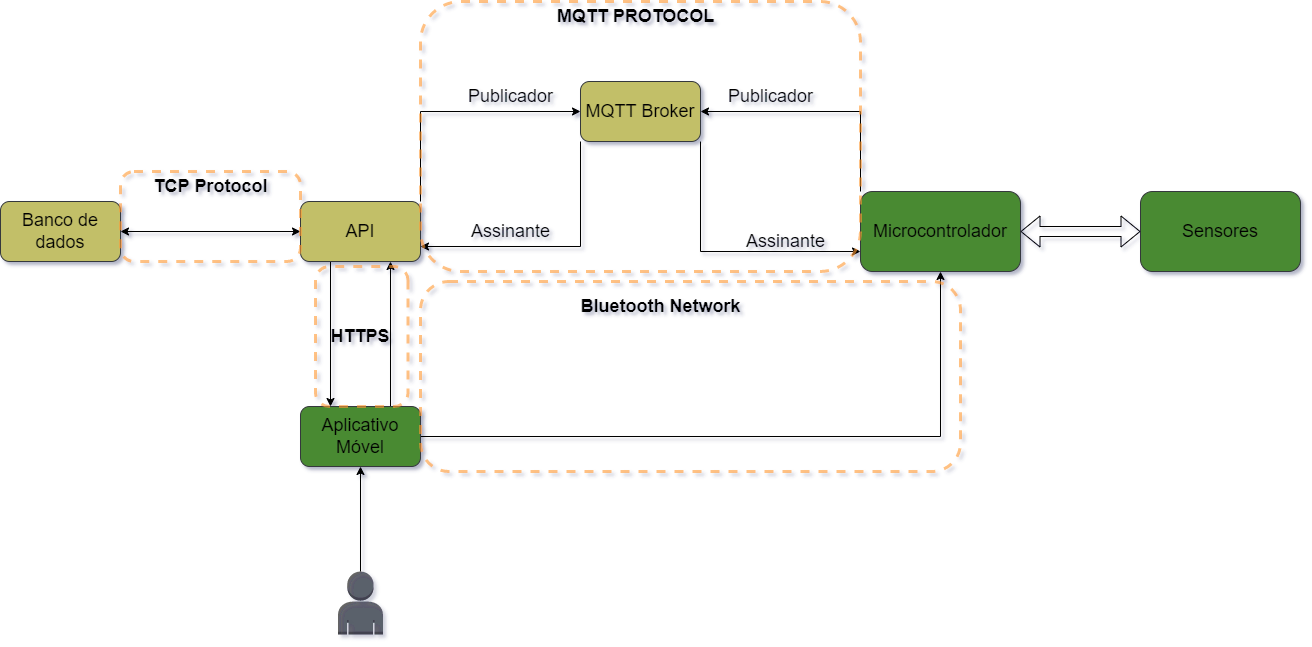
\includegraphics[width=10cm]{architecture_proj.png}
    \caption{Arquitetura do sistema proposto.}
    \label{fig:architecture}
\end{figure}

O primeiro ponto de interação ocorre através do aplicativo móvel. Neste, o usuário poderá se cadastrar para iniciar seus cuidados com a planta, poderá cadastrar o dispositivo (microcontrolador) usado para gerenciamento dos sistemas de monitoramento e controle, o usuário terá acesso aos parâmetros a serem controlados da planta e gráfico diário dos parâmetros, também terá acesso a um robô onde pode ter acesso a curiosidades, auxílio no cadastro do microcontrolador e entendimento sobre os parâmetros, e por último, acesso a um mapa. Ao utilizar o aplicativo será estabelecida uma comunicação através do Bluetooth® para o envio de algumas informações (informações sobre o Wi-Fi, nome do dispositivo, informações sobre o MQTT e informações de uma chave de API utilizada) no cadastro do microcontrolador.

Todos os cadastros dos usuários, recadastro de senha dos usuários, login dos usuários, cadastro de dispositivos, comunicação com o robô e controle dos sistemas de monitoramento e controle ocorrem através de uma API, sendo esta o ponto chave do gerenciamento de todas as trocas de informações que ocorrem no sistema proposto, ela é reponsável por recuperar, cadastrar e deletar as informações no banco de dados. Ao utilizá-la, o sistema é modularizado, onde várias responsabilidades são tiradas do aplicativo móvel e tem se maior confiabilidade no sistema. Também é adicionada resiliência ao sistema através do uso de uma Plataforma como Serviço (PaaS) disponível na nuvem tanto para a API como para o banco de dados e ao utilizar instâncias privadas para cada um.

A API além de se comunicar com o aplicativo móvel através do protocolo HTTPS também se comunica com o broker do MQTT onde está disponível os tópicos (device, localization, measure e settings) para a comunicação de Publicador-Assinante tanto entre a API e o broker, como o microcontrolador e o broker. A API atua como Assinante dos tópicos: device, localization e measure, e atua como Publicador no tópico: settings. O microcontrolador atua como Publicador nos tópicos: device, localization e measure, e atua como Assinante no tópico: settings. O diagrama na Fig.~\ref{fig:mqtt_broker} ilustra a forma como ocorre essa comunicação. 

\selectlanguage{brazil}
\begin{figure}
    \centering
    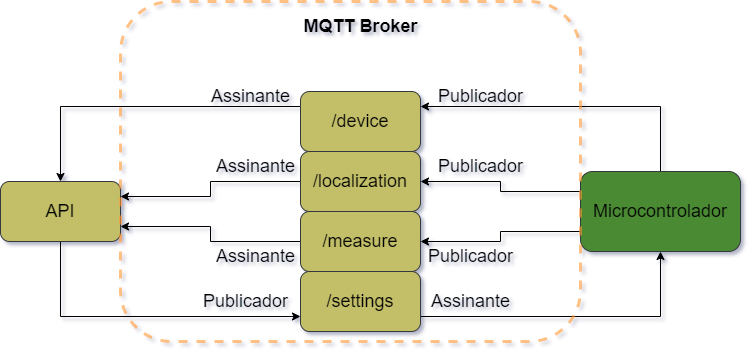
\includegraphics[width=8cm]{mqtt_broker.png}
    \caption{Diagrama da comunicação do broker com a API e o microcontrolador.}
    \label{fig:mqtt_broker}
\end{figure}

O microcontrolador se comunica com o MQTT broker para enviar os dados dos sensores do sistema de monitoramento e receber os dados para uso no sistema de controle. A Fig.~\ref{fig:sistema_controle} mostra o microcontrolador com os sensores do sistema de monitoramento e a Fig.~\ref{fig:orquidea} mostra o microcontrolador com os sensores do sistema de monitoramento na orquídea.

\selectlanguage{brazil}
\begin{figure}
    \centering
    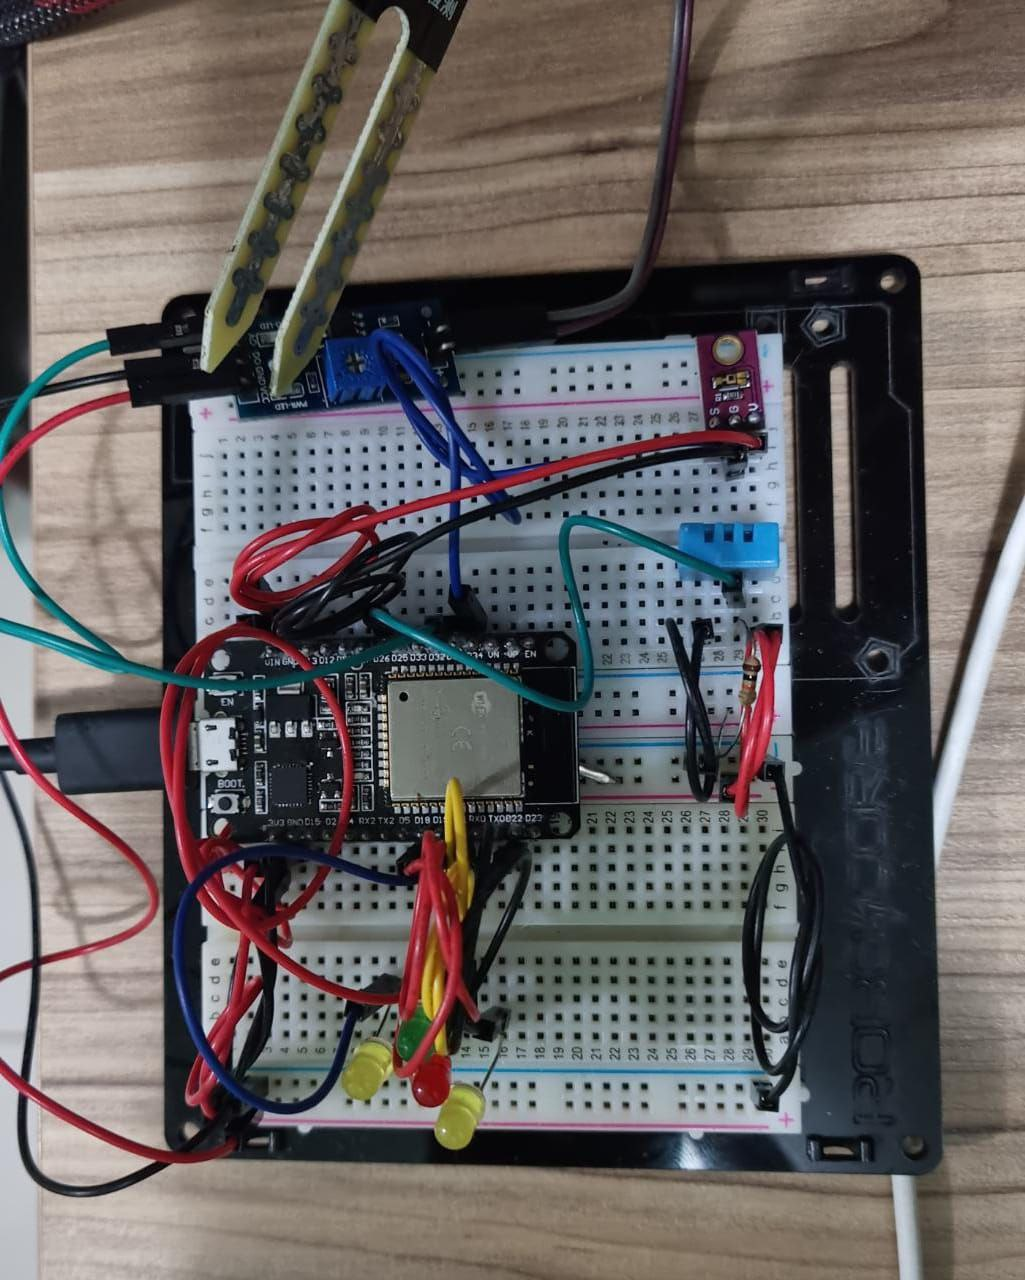
\includegraphics[width=8cm]{sistema_controle.jpg}
    \caption{Microcontrolador e sensores.}
    \label{fig:sistema_controle}
\end{figure}
\selectlanguage{brazil}
\begin{figure}
    \centering
    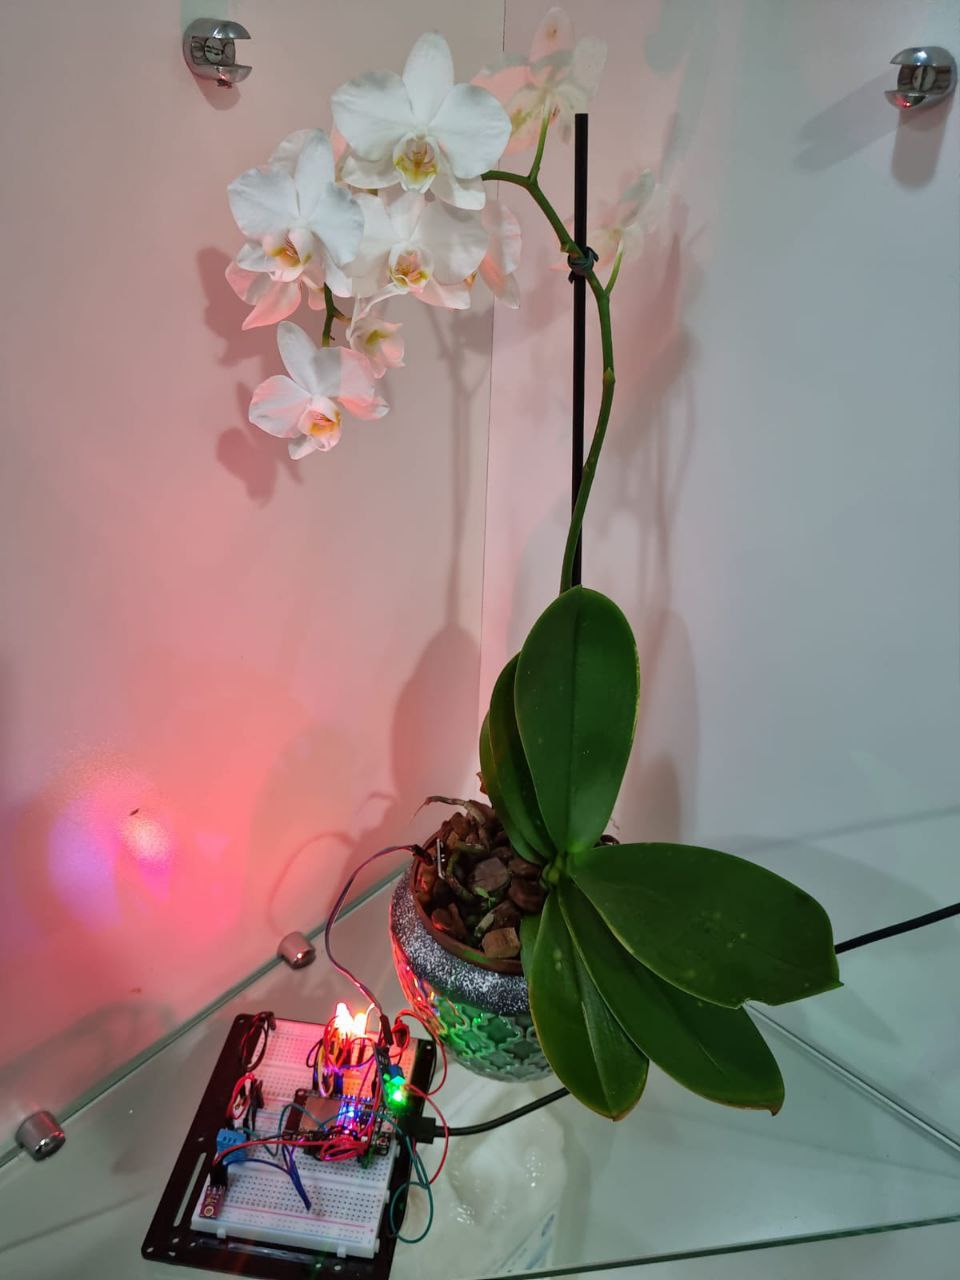
\includegraphics[width=8cm]{orquidea.jpg}
    \caption{Orquídea com microcontrolador e sensores.}
    \label{fig:orquidea}
\end{figure}

\section{Trabalhos correlatos}
O trabalho introduzido neste artigo é relacionado a Internet das Coisas, Jardim Inteligente. Além de utilizar uma API e uma aplicação móvel. A seguir, será abordado alguns trabalhos utilizados como base para que este possa ser desenvolvido.

O sistema citado em \cite{b21} busca integrar os sensores e componentes para estatísticas em tempo real atuando em jardins. Além de utilizar o Wi-Fi para comunicação com o ESP8266. O dado é transferido direto para a aplicação móvel. O dispositivo móvel dispõe de resultados em tempo real das medidas (temperatura ambiente, temperatura do solo, umidade do ar e umidade do solo), além de dispor de histórico de perfil dos fatores conforme o tempo. 
Os sensores utilizados são: sensor de temperatura (DS18B20), sensor de temperatura e umidade(DHT11) e sensor de umidade do solo (YL-69).

O sistema utilizado em \cite{b10} compõe-se de um Microcontrolador Arduino UNO, Sensor de temperatura e umidade (DHT11), Sensor de umidade do solo (SM100) e aplicação móvel. O sistema se propõe a controlar e monitorar todos os parâmetros como temperatura, umidade, umidade do solo, e intensidade de luz. A aplicação móvel disponibiliza as informações da temperatura ambiente, umidade do ar e umidade do solo. Além disso, o sistema possui módulos de controle. O sistema funciona da seguinte forma: Primeiro se inicializa o aplicativo e se conecta ao dispositivo, assim que conectado coleta-se os dados sobre a umidade do solo, e aciona o módulo para molhar a planta caso o nível de umidade não esteja normal conforme o parâmetro passado, seguidamente coleta os dados da temperatura, e aciona o módulo de ventilação caso o valor de temperatura não esteja normal, posteriormente coleta os dados da umidade do ar e aciona o módulo de luz caso a umidade não esteja normal conforme os parâmetros passados, e mostra os resultados no aplicativo.

\section{Metodologia}
Para se ter conhecimento dos parâmetros e fatores pré-colheita das orquídeas, e entender como eles influenciam no crescimento da planta foi utilizada da pesquisa bibliográfica voltada a área de biologia, especificamente orquídeas. Também utilizou-se deste tipo de pesquisa para melhor entendimento dos componentes do sistema e da comunicação utilizada no MQTT. Porém, antes do uso da pesquisa bibliográfica para entendimento dos componentes do sistema, foi necessária pesquisa exploratória e o conhecimento dos requisitos do projeto para poder construir o sistema.

\section{Resultados obtidos}
No desenvolver do sistema foram obtidos os parâmetros base para contribuição nos dados e uso no sistema proposto. Foi possível obter medições dos parâmetros (umidade do solo, umidade do ar, temperatura e incidência da luz) pelos sensores do sistema de monitoramento. Foi possível mandar os comandos para o sistema de controle de forma correta para regulação dos parâmetros através do componente de luminosidade, componente de ventilação e a bomba d'água. Foi possível visualizar tanto as medições dos parâmetros feitas pelos sensores assim como o histórico de medições no aplicativo móvel. Incorreu no sucesso do uso da API para coleta e armazenamento dos dados no banco de dados para utilização na comunicação com o microcontrolador e com a aplicação móvel. Verifica-se sucesso também na comunicação do aplicativo móvel com a API, a API com o broker do MQTT e o broker do MQTT com o microcontrolador. 

\section{Conclusão}
A Internet das coisas faz-se necessária na automação de atividades para facilitar em certas atividades que necessitam de intervenção humana, mas através de sensores, microcontroladores e sistemas pode ser diminuída a necessidade da intervenção humana, e decorrer do êxito nessas atividades.
As plantas e jardins necessitam de elevado cuidado e atenção humana para seu desenvolvimento. Porém, com o uso da Internet das coisas, e microcontroladores e sensores pode-se diminuir a carência da intervenção humana nesse cuidado, principalmente, relacionado a alguns parâmetros.

Diversos trabalhos buscaram propor sistemas nesse quesito, um para monitoramento e visualização de estatísticas dos parâmetros observados, e outro para visualização e gerenciamento de um sistema de controle para regulação desses parâmetros.

As principais contribuições deste trabalho consistem na revisão dos parâmetros e fatores essenciais para o auxílio no cuidado da Orquídea {\itshape{Phalaenopsis}}, revisão da comunicação Publicador-Assinante, construção de um sistema para monitoramento e um sistema de controle para regulação dos parâmetros da planta, e construção dos demais componentes para o uso dos que têm interesse em um maior cuidado efetivo de suas orquídeas.

Apesar das contribuições e desenvolvimentos estabelecidos neste projeto, torna-se interessante relatar possíveis desenvolvimentos futuros na continuação deste trabalho, como aprimorar a visualização dos dados, onde o usuário terá mais controle, adicionar o uso de um sistema de sugestão de acordo com os parâmetros da planta, desenvolvimento de uma rede neural para previsão da saúde da planta, e notificação do aplicativo para quando os parâmetros estiverem baixos.

\begin{thebibliography}{00}
\bibitem{b1} Verma, J. and Singh, P.,``Post-harvest Handling and Senescence in Flower Crops: An Overview,'' Agricultural Reviews. 2021.
\bibitem{b2} Augusto Porto Oliveira, Alfredo e Simone de Castro Pereira Brainer, Maria, `` Floricultura: Caracterização e Mercado,'' Documentos do Etene, Escritório Técnico de Estudos Econômicos do Nordeste, Nº 16, Banco do Nordeste, Fortaleza, 2007.
\bibitem{b3} Mattiuz, Ben-Hur. ``Fatores da pré-colheita influenciam a qualidade final dos produtos,'' Visão Agrícola nº7, Revista Visão Agrícola, USP, 2007, pp. 18--21.
\bibitem{b4} De, L.C. and Singh, D.R., ``Post –Harvest Management And Value Addition In Orchids,'' Dynamic Network for Research Works, DNetRW, International Journal of Biological Sciences, IJBS, India, 2016.
\bibitem{b5} L.C. De, Vij SP and Medhi RP, ``Post-Harvest Physiology and Technology in Orchids,'' Journal of Horticulture, India, 2014.
\bibitem{b6} G. Lopez, Roberto and S. Runkle, Erik, ``Environmental Physiology of Growth and Flowering of Orchids,'' Department of Horticulture, Michigan State University, East Lansing, 2005.
\bibitem{b7} De, Lakshman Chandra. ``Good Agricultural Practices of Commercial Orchids, '' Vigyan Varta 1(5): 53-64, 2020.
\bibitem{b8} Alexander Maier, Andrew Sharp and Yuriy Vagapov, ``Comparative Analysis and Practical Implementation
of the ESP32 Microcontroller Module for the Internet of Things,'' School of Applied Science, Computing and Engineering, Glyndwr University, UK, IEEE, 2017.
\bibitem{b9} Gondchawar, Nikesh and S. Kawitkar, Prof. Dr. R., ``IoT based Smart Agriculture,'' International Journal of Advanced Research in Computer and Communication Engineering, 5(6), India, June, 2016.
\bibitem{b10} Vinoth Kumar.P, K.C Ramya, Abishek.J.S, Arundhathy.T.S, Bhavvya.B, Gayathri.V, ``Smart Garden Monitoring and Control System with Sensor Technology,''  Department of Electrical and Electronics Engineering, Sri Krishna College of Engineering and Technology, Kuniamuthur Coimbatore, India, 2021.
\bibitem{b11} Monica M, B.Yeshika, Abhishek G.S, Sanjay H.A, Sankar Dasiga, ``IoT Based Control and Automation of Smart Irrigation System, An Automated Irrigation System Using Sensors, GSM, Bluetooth and Cloud Technology,'' Proceeding International conference on Recent Innovations is Signal Processing and Embedded Systems, NitteMeenakshi Institute of Technology, Bangalore, India., 2017.
\bibitem{b12} Lauren Murphy, Tosin Alliyu, Andrew Macvean, Mary Beth Kery, Brad A. Myers, ``Preliminary Analysis of REST API Style Guidelines,'' PLATEAU’17, Vancouver, CA, October 23, 2017.
\bibitem{b13} Surwase, Vijay, ``REST API Modeling Languages - A Developer’s Perspective,'' IJSTE - International Journal of Science Technology & Engineering, 2(10), April, 2010.
\bibitem{b14} Ram Naresh Thakur, U. S. Pandey, Jyotir Moy Chatterjee, ``Study of Mobile Application Development using MVC Framework,''Journal of Information Communication Technology and Digital Convergence, 4(2), December, 2019, pp. 13-17. 
\bibitem{b15} Singh, Mr. Siddharth, ``MVC Framework: A Modern Web Application Development Approach and Working,'' International Research Journal of Engineering and Technology (IRJET), 7(1), January, 2020.
\bibitem{b16} Meng Ma, Jun Yang, Ping Wang, Weijie Liu and Jingzhuo Zhang, ``Light-weight and Scalable Hierarchical-MVC
Architecture for Cloud Web Applications,'' IEEE, 2019.
\bibitem{b17} ``TEMT6000, Ambient Light Sensor Datasheet,'' Vishay Semiconductors, July, 2004.
\bibitem{b18} Alves Mendes Júnior, José Jair e Stevan Junior, Sérgio Luiz, ``LDR E SENSORES DE LUZ AMBIENTE: FUNCIONAMENTO E APLICAÇÕES,'' Semana de Eletrônica e Automação, Universidade Tecnológica Federal do Paraná - UTFPR, 2013.
\bibitem{b19} L. Gökrem, M. Durgun and Y. Durgun, ``Indoor Location Control with Visible Light Communication,'' 2019 3rd International Conference on Advanced Information and Communications Technologies (AICT), 2019, pp. 314-316, doi: 10.1109/AIACT.2019.8847765.
\bibitem{b20} W. Houser (2019), Kevin, ``Footcandles or Lux in IES Publications?,'' LEUKOS, 15:4, 249-250, DOI: 10.1080/15502724.2019.1638146.
\bibitem{b21} Ali, Mubashir & Kanwal, Nosheen & Hussain, Aamir & Samiullah, Fouzia & Iftikhar, Aqsa & Qamar, Mehreen. (2020). IoT Based Smart Garden Monitoring System using NodeMCU Microcontroller. International Journal of ADVANCED AND APPLIED SCIENCES. 7. 117-124. 10.21833/ijaas.2020.08.012. 
\bibitem{b22} S. Quincozes, T. Emilio and J. Kazienko, "MQTT Protocol: Fundamentals, Tools and Future Directions," in IEEE Latin America Transactions, vol. 17, no. 09, pp. 1439-1448, September 2019, doi: 10.1109/TLA.2019.8931137.
\bibitem{b23} Soni, Dipa & Makwana, Ashwin, ``A SURVEY ON MQTT: A PROTOCOL OF INTERNET OF THINGS(IOT),'' CHARUSAT University, Gujarat, India, 2017.
\bibitem{b24} ESPRESSIF, ``ESP32-DevKitC V4 Getting Started Guide,''Espressif Systems (Shanghai) Co., Ltd, 2022. Disponível em: https://docs.espressif.com/projects/esp-idf/en/latest/esp32/hw-reference/esp32/get-started-devkitc.html. Acesso em: 16/06/2022.
\bibitem{b25} ``TEMT6000,'' ESPHome, Nabu Casa. Disponível em: https://esphome.io/cookbook/temt6000.html. Acesso em: 16/06/2022.
\bibitem{b26} ``DHT11–Temperature and Humidity Sensor,'' Components101, 2021. Disponível em: https://components101.com/sensors/dht11-temperature-sensor. Acesso em: 16/06/2022.
\bibitem{b27} Silva da Cruz, Raiane; Santos de Carvalho, Ana Luísa; Cajy Silva, Leonilton; Magalhães Pereira, Rafael; Berton Zanchi, Fabrício, ``CALIBRAÇÃO DO SENSOR YL - 69 PARA FINS DE
MONITORAMENTO DA UMIDADE DE COMPOSTEIRAS,'' IV Encontro Internacional de Jovens Investigadores, 2019. Disponível em: https://editorarealize.com.br/artigo/visualizar/57524. Acesso em: 16/06/2022.
\bibitem{b28} Thomas Welsh and Elhadj Benkhelifa. 2020. On Resilience in Cloud Computing: A Survey of Techniques across the Cloud Domain. ACM Comput. Surv. 53, 3, Article 59 (May 2021), 36 pages. https://doi.org/10.1145/3388922
\bibitem{b29} Heuchert, S., Rimal, B.P., Reisslein, M. and Wang, Y. (2021), "Design of a small-scale and failure-resistant IaaS cloud using OpenStack", Applied Computing and Informatics, Vol. ahead-of-print No. ahead-of-print. https://doi.org/10.1108/ACI-04-2021-0094

\end{thebibliography}

\end{document}